\scanpage{8}
\[
\left\{\ w_0\in E_{c(\nu)}\right.
\]

\uline{Lemme} Soit $1\leq r\leq\nu$, et soit $W^{(\nu,r)}$ le quotient de $W^{(\nu)}$ par l'idéal engendré par $\dot{\Theta}_1,\ldots,\dot{\Theta}_r$. \deleted{Alors le} Soit $\deleted{\unsure{A}}\ I_{\nu,r}$ l'idéal de $A^{(\nu)}$ engendré par $\Theta_0,\ldots,\Theta_r$, de sorte que $A^{(\nu)}/I_{\nu,r}\simeq W^{(\nu,r)}$\figure{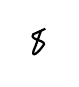
\begin{tikzpicture}[x=.14cm,y=.14cm]\draw[thick] (.8,2)--(-.3,1.5) .. controls (-.7,.9) and (1.2,1) .. (.55,.4) .. controls (-.1,-.5) and (-.6,-.6) .. (-.1,.4)--(.4,1.8);\end{tikzpicture}}. Pour que $\sum w_a\Theta_0^{a_0}\cdots\Theta_\nu^{a_\nu}$ soit dans $I_{\nu,r}$, il f. et s. que

a) pour tt \deleted{$\alpha,\ 1\leq\alpha\leq\nu-r$, \unsure{pour un}} \inserted{$a=(a_0,\ldots a_\nu)\ne0$,} \deleted{\unsure{si}} si $a_i$ est la première composante non nulle et si $i>r$, on ait $\deleted{\unsure{p}}$
\[
w_a\in p^{i-r}W
\]
b) On ait
\[
w_0\in p^{c(\nu)-r}W
\]

\uline{Cor.} Forme normale d'un élément de $W^{(\nu,r)}$ :
\[
\sum w_{a_{r+1},\ldots,a_\nu}\Theta_{r+1}^{a_{r+1}}\cdots\Theta_\nu^{a_\nu}
\]
avec
\[
\left\{\begin{aligned}
&w_{a_{r+1},\ldots a_\nu}\in E_i\deleted{\unsure{-r}}\quad\text{si }a_{r+i}\text{ est le premier des }a_\alpha\text{ qui est }\ne0\\
&w_0\in E_{c(\nu)-r}
\end{aligned}\right.
\]
\mspage{7}
